\section{四个物理见证：从可以影响，到值得改变}
\subsection{直接看不见的电流，能通过保留空间返回}
在受控的$5^3,6^3,7^3$三维矢量Maxwell网格上，构造直接输出落入接收数值零空间的两列电流。$\|SC\|$低于$1.7\times10^{-16}$，但反馈后的$\|S\bar C\|$分别为0.0672、0.0720、0.0888，指定增广带来的材料导数变化为3.56\%、3.98\%、5.22\%。新增方向本身几乎不辐射到接收器，但它激发保留电流，后者辐射到接收器。这就是接收暗电流（receiver-dark current）仍可改变材料导数的明确路径。

\begin{figure}[htbp]\centering\includegraphics[width=.9\linewidth]{figures/path_depth_dark.pdf}
\caption{直接输出和反馈后输出是不同对象。这个图检验受控物理通路，并不证明所有暗电流值得保留。}
\end{figure}

\subsection{信息更多，实际步仍可能更差}
信息体积（information volume）和有效维数（effective dimension）是材料响应谱的两个汇总量。固定正尺度$P_0$，设$\nu_i$为$P_0^{-1/2}J_U^TJ_UP_0^{-1/2}$的特征值，定义
\[
\mathcal D(U)=\tfrac12\sum_i\log(1+\nu_i),\qquad
d_{\rm eff}(U)=\sum_i\frac{\nu_i}{1+\nu_i}.
\]
它们回答模型在这个尺度下有多少、多强的材料响应。这里用$P_0=10^{-5}I$；没有实测噪声协方差标定，因此不把数值直接当成硬件互信息。信息保真度（information fidelity）另问这个曲率离完整模型有多远。这里的离线指标为$e_I(U)=\|(\mathsf I_F+P_0)^{-1/2}(\mathsf I_U-\mathsf I_F)(\mathsf I_F+P_0)^{-1/2}\|_2$，其中$\mathsf I_U=J_U^TJ_U$、$\mathsf I_F=J_F^TJ_F$；它衡量相对完整曲率的归一化误差，越小越接近。

一个近接触Maxwell对象的$k=4$替换得到$\Delta\mathcal D=6.3127$、$\Delta d_{\rm eff}=1.8613$，某个曲率保真度指标还略有改善，但完整收益$Q=-5.5754\times10^{-5}$。这一步反而更不忠实于完整GN目标。原因应从$\Delta h$与$\Delta\mathsf I s_o$的共同作用分析，不能仅凭这个见证说常数项单独导致失败。信息量描述响应；当前残差决定需要哪种响应。

\subsection{单独不利的方向，联合可能有利}
同一个rank14核心上，分别添加两列的收益为$Q_A=-3.2391\times10^{-8}$和$Q_B=-5.8389\times10^{-8}$，联合添加到rank16却得到$Q_{AB}=3.4787\times10^{-7}$。预先固定的540个pair测试中，有5个满足这种模式。配对相互作用（pair interaction）说明作用不一定可按单列相加；这些添加并非同秩交换，也不能据此推出所有Maxwell问题的普遍非次模定理。

\begin{figure}[htbp]\centering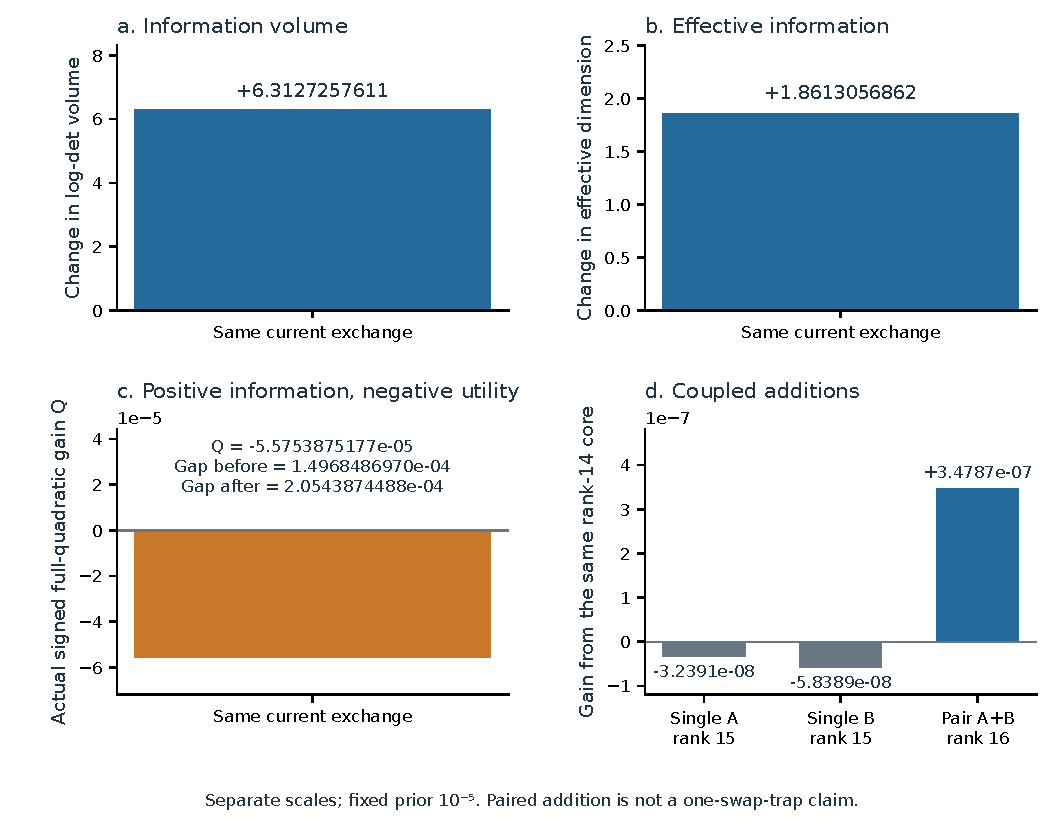
\includegraphics[width=\linewidth]{figures/information_and_pair_witness.pdf}
\caption{左侧说明信息体积及有效维数上升不足以判断实际收益，右侧展示同一核心的两单列与联合添加。各量使用自己的单位。}
\end{figure}

\subsection{必须评价真实位移的有限代价}
受控诊断使用同一批候选，分开位移构造和收益评价。$v$是旧曲率给出的一阶近似位移（first-order displacement），$d=s_n-s_o$是实际端点位移（actual endpoint displacement）；每种位移分别用线性项或完整二次式排序，最后统一执行真实$d$。

故意移除no-op、强制选择top-one时，$-g_F^Td$在29/36单元挑中负收益，加入$-\tfrac12d^TH_Fd$以后只有1/36。有限位移的曲率代价（finite-displacement curvature cost）确实改变候选排序。部署程序仍有no-op和真实$Jd$复核；上述计数是诊断结果，不是部署失败率。
